\documentclass{article}

% if you need to pass options to natbib, use, e.g.:
%     \PassOptionsToPackage{numbers, compress}{natbib}
% before loading neurips_2019

% ready for submission
% \usepackage{neurips_2019}

% to compile a preprint version, e.g., for submission to arXiv, add add the
% [preprint] option:
%     \usepackage[preprint]{neurips_2019}

% to compile a camera-ready version, add the [final] option, e.g.:
\usepackage[]{neurips_2019}

% to avoid loading the natbib package, add option nonatbib:
%     \usepackage[nonatbib]{neurips_2019}

\usepackage[utf8]{inputenc} % allow utf-8 input
\usepackage[T1]{fontenc}    % use 8-bit T1 fonts
\usepackage{hyperref}       % hyperlinks
\usepackage{url}            % simple URL typesetting
\usepackage{booktabs}       % professional-quality tables
\usepackage{amsfonts}       % blackboard math symbols
\usepackage{nicefrac}       % compact symbols for 1/2, etc.
\usepackage{microtype}      % microtypography
\usepackage{graphicx}       % images
\usepackage{float}          % image positioning
\usepackage{subfig}         % image positioning

\title{Reproduction of GANSpace}

% The \author macro works with any number of authors. There are two commands
% used to separate the names and addresses of multiple authors: \And and \AND.
%
% Using \And between authors leaves it to LaTeX to determine where to break the
% lines. Using \AND forces a line break at that point. So, if LaTeX puts 3 of 4
% authors names on the first line, and the last on the second line, try using
% \AND instead of \And before the third author name.

\author{%
  David S.~Hippocampus\thanks{Use footnote for providing further information
    about author (webpage, alternative address)---\emph{not} for acknowledging
    funding agencies.} \\
  Department of Computer Science\\
  Cranberry-Lemon University\\
  Pittsburgh, PA 15213 \\
  \texttt{hippo@cs.cranberry-lemon.edu} \\
  % examples of more authors
  % \And
  % Coauthor \\
  % Affiliation \\
  % Address \\
  % \texttt{email} \\
  % \AND
  % Coauthor \\
  % Affiliation \\
  % Address \\
  % \texttt{email} \\
  % \And
  % Coauthor \\
  % Affiliation \\
  % Address \\
  % \texttt{email} \\
  % \And
  % Coauthor \\
  % Affiliation \\
  % Address \\
  % \texttt{email} \\
}

\begin{document}

\maketitle

\section*{\centering Reproducibility Summary}

% \textit{Template and style guide to \href{https://paperswithcode.com/rc2020}{ML Reproducibility Challenge 2020}. The following section of Reproducibility Summary is \textbf{mandatory}. This summary \textbf{must fit} in the first page, no exception will be allowed. When submitting your report in OpenReview, copy the entire summary and paste it in the abstract input field, where the sections must be separated with a blank line.}

\subsection*{Scope of Reproducibility}

% State the main claim of the original paper you are trying to reproduce. We recommend picking the central claim of the paper.
% This is meant to place the work in context, and to tell a reader the objective of the reproduction.
The authors introduce a novel approach to analyze Generative Adversarial Networks (GANs) and create interpretable controls for image manipulation and synthesis. This is done by identifying important latent directions based on Principal Component Analysis (PCA) applied either in the latent space or the feature space. We aim to validate the claims and reproduce the results in the original paper.

\subsection*{Methodology}

% Briefly describe what you did and which resources did you use. E.g. Did you use author's code, did you re-implement parts of the pipeline, how much time did it take to produce the results, what hardware you were using and how long it took to train/evaluate.
The code that was provided by the authors in Pytorch was reimplemented in \textbf{Tensorflow 1.x} for the pretrained \textit{StyleGAN} and \textit{StyleGAN2} architectures. This was done with the help of the APIs provided by the original authors of these models.
\\
The experiments were run on an Intel i7 processor containing 16 GB of RAM, coupled with an Nvidia 1060 GPU having 6 GB of VRAM.

\subsection*{Results}

% Start with your overall conclusion - where was your study successful and where not successful. Be specific and use precise language, e.g. "we reproduced the accuracy to within 1\% of reported value, that upholds the paper's conclusion that it performs much better than baselines". Getting exactly the same number is in most cases infeasible, so you'll need to use your judgement call to decide if your results support the original claim of the paper.
We were able to reproduce the results and verify the claims made by the authors for the StyleGAN and StyleGAN2 models by recreating the modified images, given the seed and other configuration parameters.
Additionally, we also perform our own experiments to identify new edits and show that edits are transferable across similar datasets using the techniques proposed by the authors.

\subsection*{What was easy}

% Describe which parts of your reproduction study were easy. E.g. was it easy to run the author's code, or easy to re-implement their method based on the description in the paper. The goal of this section is to summarize to the reader which parts of the original paper they could easily apply to their problem. 
The paper provides detailed explanations for the different mathematical concepts that were involved in the proposed method. This, augmented with a well-structured and documented code repository, allowed us to understand the major ideas in a relatively short period of time. Running the experiments using the original codebase was straightforward and highly efficient as well, as the authors have taken additional steps to employ batch processing wherever possible.

\subsection*{What was difficult}

% Describe which parts of your reproduction study were difficult or took much more time than you expected. Perhaps the data was not available and you couldn't verify some experiments, or the author's code was broken and had to be debugged first. Or, perhaps some experiments just take too much time/resources to run and you couldn't verify them. The purpose of this section is to indicate to the reader which parts of the original paper are either difficult to re-use, or require a significant amount of work and resources to verify.
Originally we were attempting to recreate identical images with zero delta in the RGB values. However, due to differences in the random number generators between PyTorch-CPU, PyTorch-GPU and Numpy, the random values were not the same even with the same seed. This resulted in minute differences in the background artifacts of the generated images. Additionally, there is a lack of open source Tensorflow 1.x APIs to access the intermediate layers of the \textit{BigGAN} model. Due to time constraints, we were unable to implement these accessors and verify the images that the authors of GANSpace created using \textit{BigGAN}.

\subsection*{Communication with original authors}

% Briefly describe how much (if any contact) you had with the original authors.
While conducting our experiments, we did not contact the original authors. The paper and codebase were organized well and aided us in effectively reproducing and validating the authors' claims.

\newpage
% \textit{\textbf{
% The following section formatting is \textbf{optional}, you can also define sections as you deem fit.
% \\
% Focus on what future researchers or practitioners would find useful for reproducing or building upon the paper you choose.
% }}
\section{Introduction}
% A few sentences placing the work in context. Limit it to a few paragraphs at most; your report is on reproducing a piece of work, you don’t have to motivate that work.

Generative Adversarial Networks (GANs) \cite{gan} are a type of machine learning framework where two neural networks, the discriminator and the generator, compete with each other in a zero-sum game. The generator tries to trick the discriminator into believing that artificially generated samples belong to real data.

GANs have proven to be powerful image synthesis tools, which are capable of producing high quality images. However, they provide little control over the features of the generated image. Existing solutions to add user control over the generated images require expensive supervised training on latent vectors.

GANSpace \cite{ganspace} proposes a simple technique to discover interpretable GAN controls in a unsupervised manner. The authors show that important directions in the latent space that affect the output can be identified using Principal Component Analysis (PCA). Their experiments on StyleGAN \cite{stylegan}, StyleGAN2 \cite{stylegan2} and BigGAN512-deep \cite{biggan} demonstrate that layer-wise decomposition of PCA directions leads to many interpretable controls, which affects both low and high level attributes of the output image.


\section{Scope of reproducibility}
\label{claims}

% Explain the claims from the paper you picked for the reproduction study and briefly motivate your choice. We recommend picking the claim that is the central contribution of the paper. To find what this contribution is, try to summarize the most important result of the paper in 1-2 sentences, e.g. "This paper introduces a new activation function X that outperforms a similar activation function Y on tasks Z,V,W". 

For our reproduction study, we aim to validate the effectiveness of the proposed technique in offering powerful interpretable controls on the output images in an unsupervised manner.

% Make the scope as specific as possible. It should be something that can be supported or rejected by your data. For example, this scope is too broad and lacks precise outcome (what is "strong performance"?): "Contextual embedding models have shown strong performance on a number of tasks across NLP. We will run experiments evaluating two types of contextual embedding models on datasets X, Y, and Z."

% This scope is better because it's more specific and has an outcome that can be either supported or rejected based on your work: "Finetuning Pretrained BERT on SST-2 will have higher accuracy than an LSTM trained with GloVe embeddings."
% 2.1 Addressed claims from the original paper

The following claims of the paper have been verified and tested successfully:
\begin{itemize}
    \item PCA can be used to highlight important directions in the GAN's latent space.
    \item The GAN's output can be controlled easily in an unsupervised fashion.
    \item The earlier components control the higher-level aspects of an image, while the later directions primarily affect the minute details.
\end{itemize}


\section{Methodology}

% Explain your approach - did you use the author's code, did you aim to re-implement the approach from the paper description. Summarize the resources (code, documentation, GPUs) that you used. 

% We used the author's code while running our experiments. The code was modified to support the StyleGAN and StyleGAN2 Tensorflow 1.x APIs.

The output of StyleGAN and StyleGAN2 can be controlled by identifying principal axes of $p(\textbf{w})$, which is the probability distribution of the output of the mapping network $M$. First, we sample $N$ latent vectors $\textbf{z}_{1:N}$ and compute the corresponding $\textbf{w}_{i} = M(\textbf{z}_{i})$. The PCA of these $\textbf{w}_{1:N}$ values gives us the basis $\textbf{V}$ for $\mathcal{W}$. The output attributes of a new image given by $\textbf{w}$ can then be controlled by varying the PCA coordinates of \textbf{x} before feeding them into the synthesis network.

\begin{equation}
    \textbf{w'} = \textbf{w} + \textbf{Vx}
\end{equation}

Each entry $x_{k}$ of \textbf{x} is a separate control parameter which can be modified to update the desired attributes of the output image.

We follow the same notation used by the authors to denote edit directions in this report. $E(\textbf{v}_{i}, j-k)$ means moving along component $v_{i}$ from layers $j$ to $k$.

\subsection{Model descriptions}
% Describe the models used in the original paper, if you implemented them yourself or used the author's code. Be sure to list the type of model, the number of parameters, and other relevant info (e.g. if it's pretrained).

We use NVIDIA's official implementation of StyleGAN \footnote{\url{https://github.com/NVlabs/stylegan}} and StyleGAN2 \footnote{\url{https://github.com/NVlabs/stylegan2}} models. The authors code for computing PCA on the latent space of StyleGAN was modified to support the API's provided by NVIDIA.

\subsection{Datasets}
% Describe the datasets you used and how you obtained them. For each dataset include 1) relevant statistics such as the number of examples and label distributions, 2) details of train / dev / test splits, 3) an explanation of any preprocessing done, and 4) a link to download the data (if available).

The experiments in the paper were performed using the FFHQ, LSUN Car, CelebAHQ, Wikiart, Horse and Cat datasets. The official Tensorflow implementation of StyleGAN contains links to download pretrained models on FFHQ, LSUN Car, Wikiart, Horse and Cat. The models trained on Wikiart were downloaded from awesome-pretrained StyleGAN \footnote{\url{https://github.com/justinpinkney/awesome-pretrained-stylegan}}.

In addition to the datasets using by the authors, we also perform our own experiments on the Beetles and Anime datasets which were downloaded from awesome-pretrained StyleGAN2 \footnote{\url{https://github.com/justinpinkney/awesome-pretrained-stylegan2}}.

% \subsection{Hyperparameters}
% Describe how you set the hyperparameters and what was the source for their value (e.g. paper, code or your guess). If there was a hyperparameter search done, be sure to include the range of hyperparameters searched over, the method used to search (e.g. manual search, random search, Bayesian optimization, etc.), and the best hyperparameters found. Include the number of total experiments (e.g. hyperparameter trials). You can also include all results from that search (not just the best-found results).

\subsection{Experimental setup}
% Explain how you ran your experiments, e.g. the CPU/GPU resources and provide the link to your code and notebooks. Include a description of the specific measure used to evaluate the experiments (e.g. accuracy, precision@K, BLEU score, etc.).

All the experiments were conducted on a laptop with an Intel i7 8750H processor, 16GB RAM, NVIDIA GTX 1060 6 GB GPU and Ubuntu 18.04. The generated images from our experiments were evaluated visually to determine whether the edits were working as expected.


% \subsection{Computational requirements}
% All our experiments are computationally inexpensive.
% Provide information on computational requirements for each of your experiments. For example, the number of CPU/GPU hours and memory requirements. You'll need to think about this ahead of time, and write your code in a way that captures this information so you can later add it to this section.
% For each model, include a measure of the average runtime (e.g. average time to predict labels for a given validation set with a particular batch size).
% For each experiment, include the total computational requirements (e.g. the total GPU hours spent).


\section{Results}

First we validate the claims of the orignal paper mentioned in section \ref{claims}. Then we move on to provide additional results that validate the effectiveness of the technique employed by GANSpace.

% Start with a high-level overview of your results. Does your work support the claims you listed in section 2.1? Keep this section as factual and precise as possible, reserve your judgement and discussion points for the next "Discussion" section. 

% Go into each individual result you have, say how it relates to one of the claims and explain what your result is. Logically group related results into sections. Clearly state if you have gone beyond the original paper to run additional experiments and how they relate to the original claims. 

\subsection{Effectiveness of PCA}

\begin{figure}[H]
    \centering
    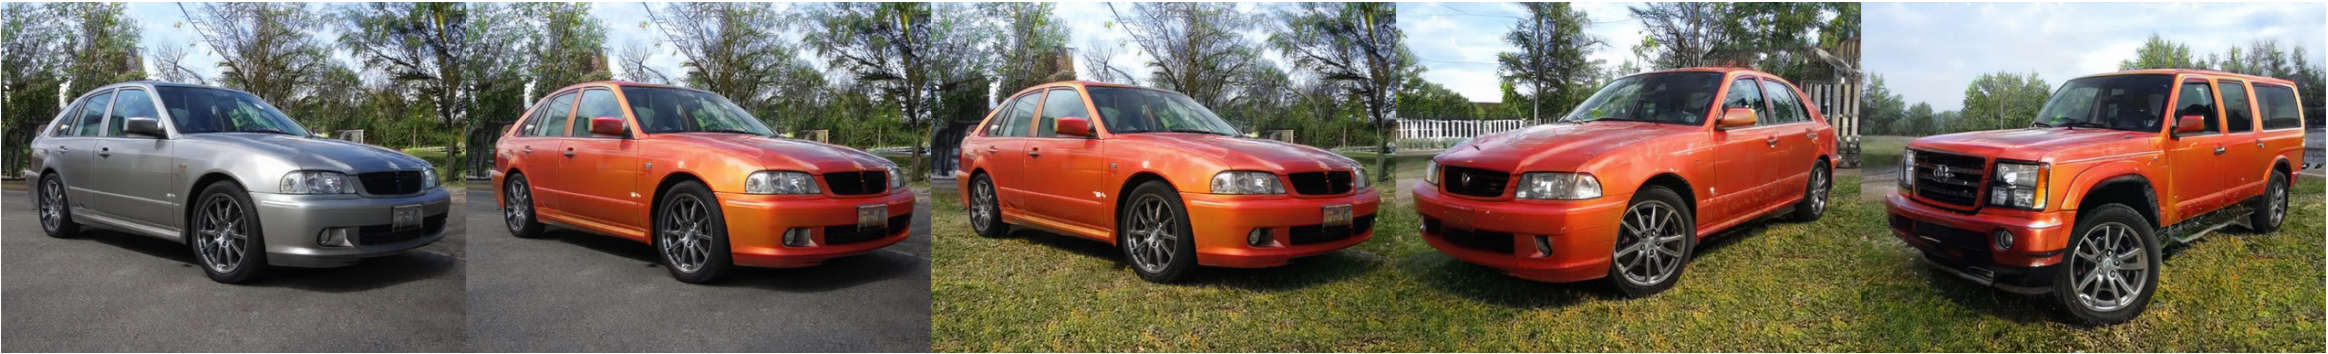
\includegraphics[width=\textwidth]{figs/figure1_StyleGAN2_cars.png}
    \caption{Sequences of image edits performed using control discovered with StyleGAN2 cars: ``Initial Image" $\rightarrow$ ``Change Color" $\rightarrow$ ``Add Grass" $\rightarrow$ ``Rotate" $\rightarrow$ "Change Type"}
    \label{fig:cars}
\end{figure}

Figure \ref{fig:cars} highlights the effectiveness of PCA on changing low and high level attributes of the image. We are able to control object shape, colour and pose as well as nuanced landscape attributes.

The edit directions corresponding to each of the edits are: $E(\textbf{v}_{22}, 9-10)$ ("Change Color"), $E(\textbf{v}_{11}, 9-10)$ ("Add Grass"), $E(\textbf{v}_{0}, 0-4)$ ("Rotate") and $E(\textbf{v}_{16}, 3-5)$ ("Change type").

\subsection{Unsupervised vs Supervised methods}

\begin{figure}[H]

\subfloat[Edit directions identified by PCA ($E(\textbf{v}_{1}, 0-1)$)]{%
  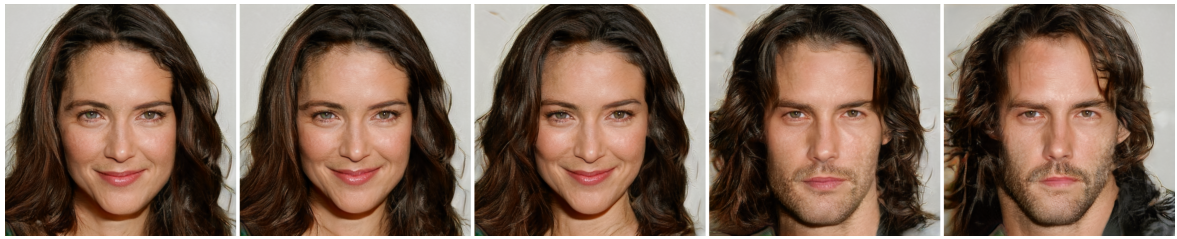
\includegraphics[clip,width=\columnwidth]{figs/figure5_gender-ours_scale=-3.2.png}%
}

\subfloat[Edit directions identified by supervised methods \cite{supervised}]{%
  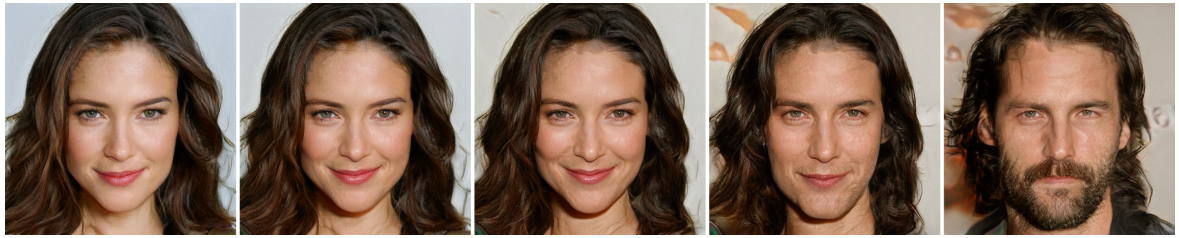
\includegraphics[clip,width=\columnwidth]{figs/figure5_gender-supervised_scale=1.2.png}%
}

\caption{Comparison of edits using unsupervised and supervised methods}

\end{figure}

The original authors point out that previous methods for finding interpretable directions in GAN latent spaces require outside supervision, such as labeled training images or pretrained classifiers, whereas GANSpace aims to automatically identify variations intrinsic to the model without supervision. This has been validated using the CelebA HQ Faces dataset by comparing the edit directions found through PCA to those found in previous work using supervised methods.

\subsection{Effect of different components}

\begin{figure}[H]
    \centering
    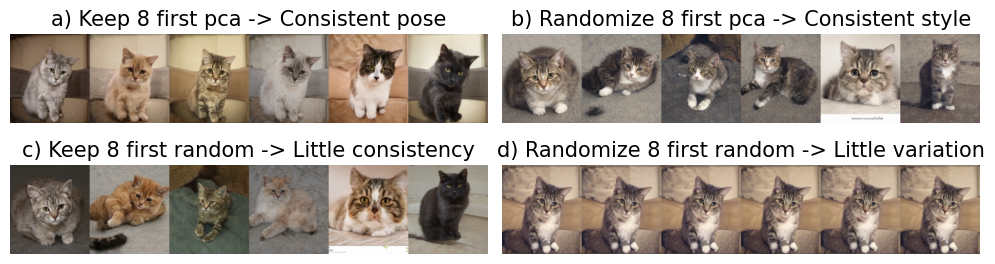
\includegraphics[width=\textwidth]{figs/figure4_randomize_8_first_random-little_variation.png}
    \caption{Illustration of the significance of the principal components as compared to random directions in the intermediate latent space of StyleGAN2.}
    \label{fig:cats}
\end{figure}

The original authors claim that the earlier components primarily control the geometry and other high-level aspects, while the lower components capture minute details. This has been illustrated in \ref{fig:cats}. Fixing and randomizing the early principal components shows a separation between pose and style. In contrast, fixing and randomizing randomly-chosen directions does not yield a similar meaningful decomposition.

\subsection{Additional results not present in the original paper}

\subsubsection{New edits}

We identify new edits on the Stylegan2 Beetles dataset. Edit $E(\textbf{v}_{2}, 0-17)$, referred to as "Patterns", adds a pattern on the shell of the beetle. The generated pattern varies depending on the seed used to sample $\textbf{w}$.

\begin{figure}[H]

\subfloat[Beetle generated with seed 1819967864]{%
  \includegraphics[clip,width=\columnwidth]{figs/figure7_beetles_pattern.png}%
}

\subfloat[Beetle generated with seed 1]{%
  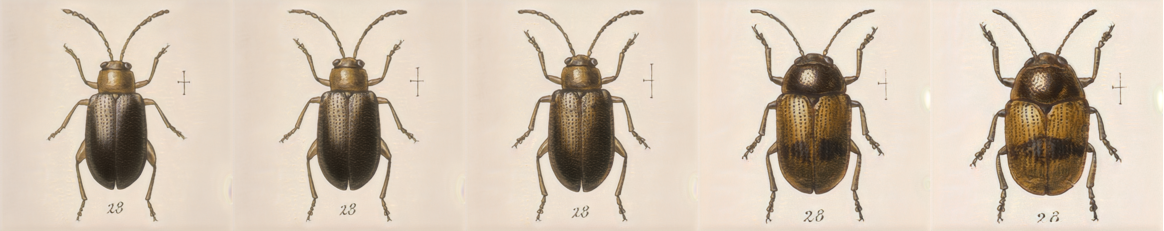
\includegraphics[clip,width=\columnwidth]{figs/figure7_different_beetle_pattern.png}%
}

\caption{"Patterns" edit applied on the output images of StyleGAN2 Beetles}

\end{figure}


\subsubsection{Transferable edits across similar datasets}

\begin{figure}[H]

\subfloat[Hair Color generated with seed 452352 on the Anime Portraits dataset]{%
  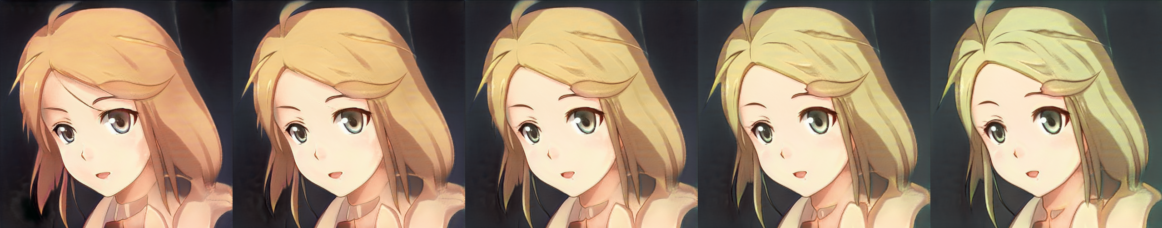
\includegraphics[clip,width=\columnwidth]{figs/figure7_anime_hair_color.png}%
}

\subfloat[Hair Color generated with seed 452352 on the FFHQ dataset]{%
  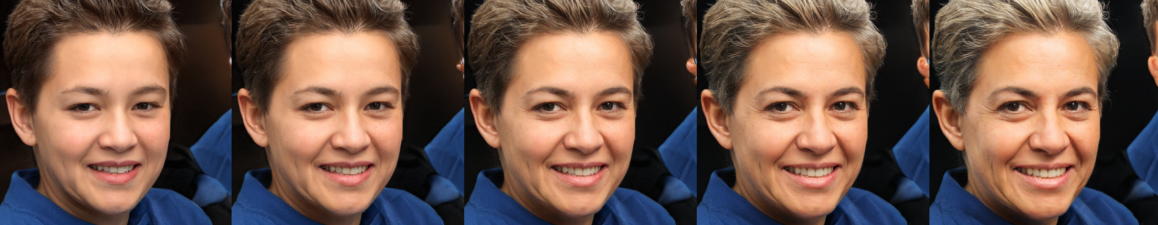
\includegraphics[clip,width=\columnwidth]{figs/figure7_human_hair_color_edits-across-datasets.png}%
}

\caption{"Hair Color" edit applied on the output images of StyleGAN2 Anime Portraits and StyleGAN2 FFHQ datasets}
\label{fig:edits_across_datasets}

\end{figure}

The original authors limit the application of edits to the same dataset. We additionally show that the edits are transferable across datasets, provided that the seed values generate similar images. This has been illustrated in \ref{fig:edits_across_datasets}.

\subsubsection{Truncation Psi on StyleGAN}

The original authors use the "truncation trick" on images generated using StyleGAN2 to improve their quality. However, this is not enabled for StyleGAN images. During our experimentation, we found that enabling truncation while applying edits on StyleGAN images improved their quality as well. We demonstrate this using the Wikiart dataset using the "Head Rotation" ($E(\textbf{v}_{7}, 0-1)$) and "Simple Strokes" ($E(\textbf{v}_{9}, 8-14)$ edits.

\begin{figure}[H]

\subfloat["Head Rotation" and "Simple Strokes" edits on StyleGAN Wikiart with truncation psi set to 0.7]{%
  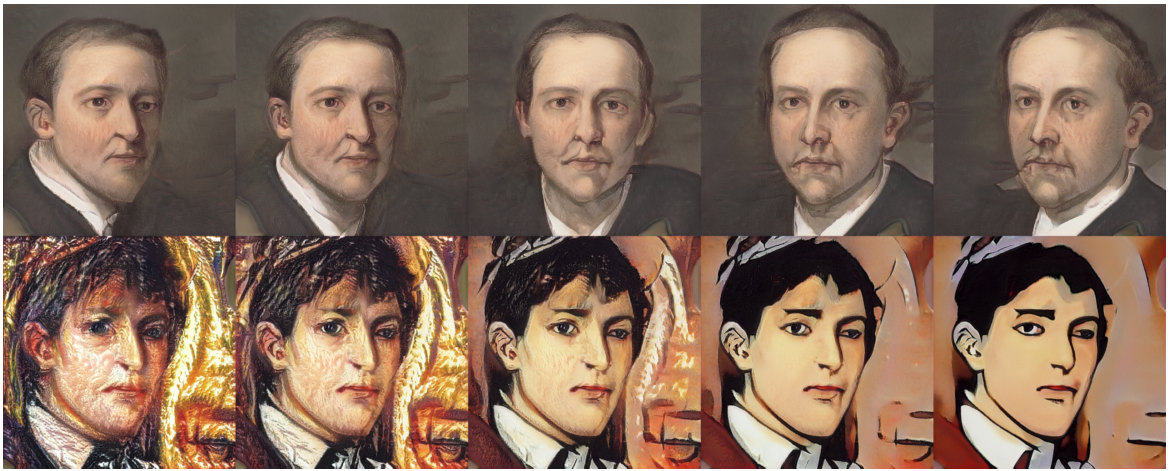
\includegraphics[clip,width=\columnwidth]{figs/figure7_StyleGAN_wikiart_truncation.png}%
}

\subfloat["Head Rotation" and "Simple Strokes" edits on StyleGAN Wikiart without truncation psi]{%
  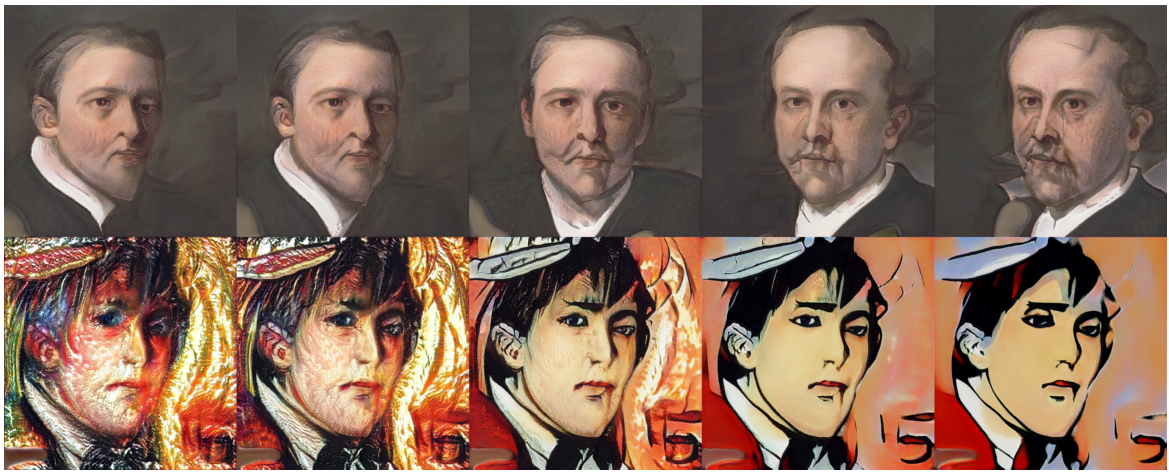
\includegraphics[clip,width=\columnwidth]{figs/figure7_StyleGAN_wikiart_Rotation_Simple-strokes.png}%
}

\caption{Quality of images generated by StyleGAN before and after applying the "truncation trick".}

\end{figure}

% \begin{figure}[H]
%     \centering
%     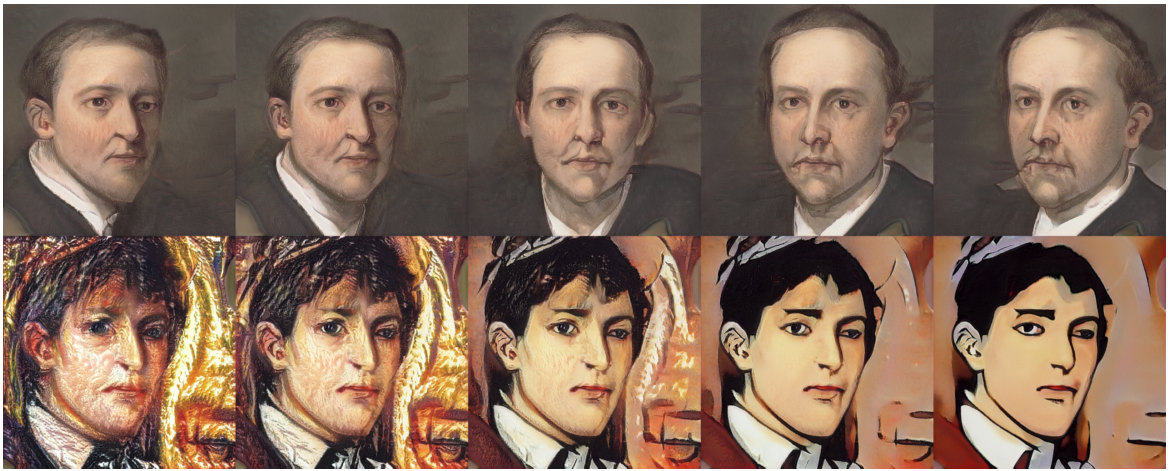
\includegraphics[width=\textwidth]{figs/figure7_StyleGAN_wikiart_truncation.png}
%     \caption{"Head Rotation" and "Simple Strokes" edits on StyleGAN with truncation psi set to 0.7}
%     \label{fig:my_label}
% \end{figure}

% \begin{figure}[H]
%     \centering
%     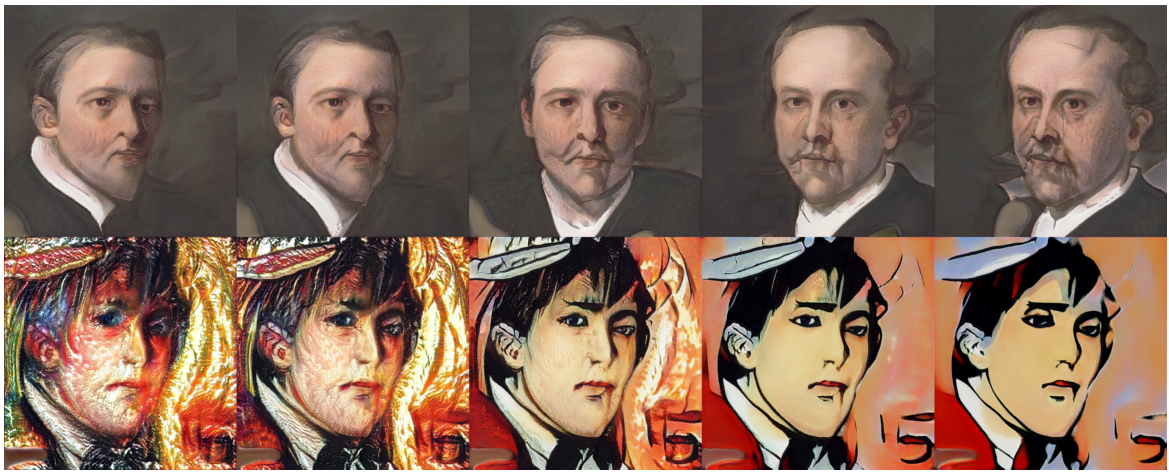
\includegraphics[width=\textwidth]{figs/figure7_StyleGAN_wikiart_Rotation_Simple-strokes.png}
%     \caption{"Head Rotation" and "Simple Strokes" edits on StyleGAN without truncation psi}
%     \label{fig:my_label}
% \end{figure}


% Often papers don't include enough information to fully specify their experiments, so some additional experimentation may be necessary. For example, it might be the case that batch size was not specified, and so different batch sizes need to be evaluated to reproduce the original results. Include the results of any additional experiments here. Note: this won't be necessary for all reproductions.

\section{Discussion}

% Give your judgement on if you feel the evidence you got from running the code supports the claims of the paper. Discuss the strengths and weaknesses of your approach - perhaps you didn't have time to run all the experiments, or perhaps you did additional experiments that further strengthened the claims in the paper.

After performing our experiments, we feel that the results justify the claims of the paper. This is further bolstered by the fact that the proposed method worked on different datasets which were not covered by the original authors.


\subsection{What was easy}
% Give your judgement of what was easy to reproduce. Perhaps the author's code is clearly written and easy to run, so it was easy to verify the majority of original claims. Or, the explanation in the paper was really easy to follow and put into code. 

Verifying the claims of the paper was easy as the author's code was well documented and clearly written. The paper was well organized and provided a lot of examples on various datasets to demonstrate exactly how their algorithm works. The authors ensured that all the figures in the paper had accompanying code to recreate them.

NVIDIA's implementation of StyleGAN and StyleGAN2 provided access to well written API's which we could integrate easily into the author's codebase. We did not have to create our own wrappers by accessing the weights of the pretrained models.

% Be careful not to give sweeping generalizations. Something that is easy for you might be difficult to others. Put what was easy in context and explain why it was easy (e.g. code had extensive API documentation and a lot of examples that matched experiments in papers). 

\subsection{What was difficult}
% List part of the reproduction study that took more time than you anticipated or you felt were difficult. 

While running our experiments, we noticed that the there was a small difference in the RGB values of the recreated images. This was due to the difference in the random values generated by PyTorch-CPU, PyTorch-GPU and Numpy random number generators even when seeded with the same seed. The noise variables in the StyleGAN networks were not identical because of this. This resulted in minute differences in background artifacts of the images.

We were not able to replicate the author's experiments on BigGAN-512 deep due to time constraints. 

% Be careful to put your discussion in context. For example, don't say "the maths was difficult to follow", say "the math requires advanced knowledge of calculus to follow". 

\subsection{Communication with original authors}
% Document the extent of (or lack of) communication with the original authors. To make sure the reproducibility report is a fair assessment of the original research we recommend getting in touch with the original authors. You can ask authors specific questions, or if you don't have any questions you can send them the full report to get their feedback before it gets published. 
While conducting our experiments, we did not contact the original authors. The paper and codebase were organized well and aided us in effectively reproducing and validating the authors' claims.


% \section*{References}

\bibliographystyle{unsrt}
\bibliography{reganspace}

\end{document}
